\documentclass[10pt]{article}
\usepackage{icmlko}

\icmlmeta{IP 파운데이션 월드모델}{134}{기준선이 처치보다 크다}{노트 133의 채택 권고를 재 보니 2x2의 한 칸이었다 --- 그리고 그 2x2 를 만든 자료 빌드 선택이 이 판에서 잰 거의 모든 처치보다 크다}

\begin{document}

\twocolumn[
\icmlheader

\begin{abstract}
노트 133이 ``학습 문턱을 40에서 15로 낮춘다''를 채택했다. 근거는 짝 순위
우도가 팝업에서 $+$0.3698에서 $+$0.4300으로 오른 것이었다. 전 판에서
재확정하려고 다시 쟀더니 \textbf{그 $+$0.060이 2$\times$2의 한 칸이었다.}
같은 처치가 팝업 빌드와 모형에 따라 부호가 뒤집힌다 --- audit 빌드에서
짝 순위는 $-$0.006, 부스팅은 $+$0.036이고, popupset 빌드에서 짝 순위는
$+$0.060, 부스팅은 $-$0.038이다. 넷 중 둘이 음수다. 그리고 \textbf{제일
높은 칸은 손 안 댄 현행}(짝 순위 · audit · 문턱 40, $+$0.4995)이다.
\textbf{더 큰 것을 봤다.} 두 팝업 빌드의 차이가 중앙 $+$0.0906인데, 이
판에서 노트 128부터 잰 처치 효과가 검색 축 $+$0.0744 · 팝업 확장 $+$0.0601 ·
문턱 $+$0.0370 · 웹툰 덮음 $+$0.0125 · 달력 축 $+$0.0096이다.
\textbf{기준선 선택 하나가 거의 모든 처치보다 크다.} 두 빌드의 차이는
노트 124가 ``사람이 안 매겼다''고 판정한 팝업 8건의 관측 표시자 하나뿐이다.
그래서 규약을 셋 고쳤다 --- 실행 이름에 설정을 다 넣고(문턱만 다른 두 실행이
같은 이름으로 저장돼 포트폴리오 최고값이 섞여 있었다), 팝업 빌드를 config에
기록하고, 하네스가 행 수 불일치를 조용히 메우지 않게 했다. 그러고 나서
부스팅 · audit · 문턱 15 가 판 $\rho$ \textbf{$+$0.4409}로 가드 여덟을
통과해 챔피언이 됐다.
\end{abstract}
]

\begin{figure*}[t]
\centering
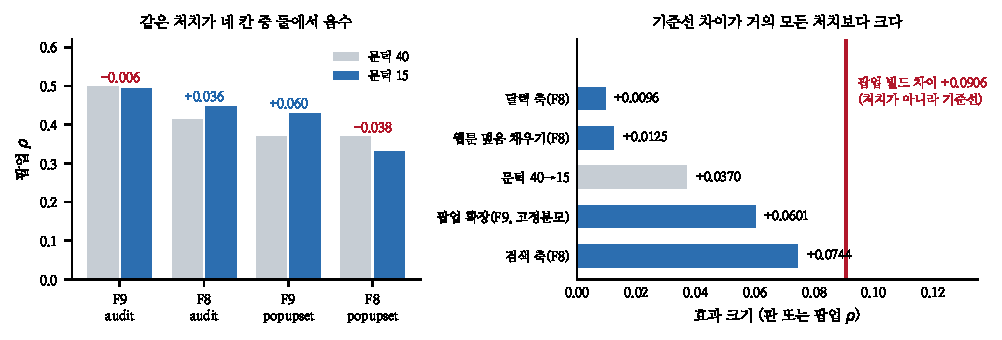
\includegraphics[width=\textwidth]{figs/base.pdf}
\caption{왼쪽 --- 같은 처치가 네 칸 중 둘에서 음수다. 오른쪽 --- 팝업 빌드
차이(붉은 선)가 이 판에서 잰 거의 모든 처치보다 크다.}
\end{figure*}

\section{한 칸을 채택했었다}

노트 133은 확장의 이득을 갈라 보고 ``주장 레코드는 필요 없다, 문턱만
낮추면 된다''로 끝냈다. 근거가 이 한 줄이었다 --- 짝 순위 우도가 좁은 판
$+$0.3698에서 문턱 15로 $+$0.4300. 전 판에서 재확정하려고 문턱을
설정 가능하게 만들고 다시 쟀다.

\begin{table}[t]
\centering\tsize
\caption{팝업 $\rho$. 축은 검색 $+$ 달력으로 고정.}
\begin{tabular}{llrrr}
\toprule
& 빌드 & 문턱 40 & 문턱 15 & 차 \\
\midrule
F9 짝 순위 & audit & \textbf{$+$.4995} & $+$.4938 & $-$.006 \\
F8 부스팅 & audit & $+$.4124 & $+$.4481 & $+$.036 \\
F9 짝 순위 & popupset & $+$.3698 & $+$.4300 & $+$.060 \\
F8 부스팅 & popupset & $+$.3690 & $+$.3307 & $-$.038 \\
\bottomrule
\end{tabular}
\end{table}

\claimx{\textbf{같은 처치가 네 칸 중 둘에서 음수다.} 그리고 제일 높은 칸은
손 안 댄 현행이다(F9 · audit · 문턱 40). 노트 133의 채택 권고는 이 표의
셋째 줄 하나였다.}{먼저 문턱 변경이 팝업 \emph{하나만} 가른다는 것을
확인했다 --- 나머지 아홉 도메인은 2025년 이전 레코드가 이미 40건 이상이다.
그래서 부작용은 없고, 다만 얻는 것도 없다.}

\section{그리고 더 큰 것을 봤다}

두 빌드의 차이가 처치보다 크다.

\begin{table}[t]
\centering\tsize
\caption{이 판에서 노트 128부터 잰 것들. 마지막 줄만 처치가 아니다.}
\begin{tabular}{lr}
\toprule
검색 축 (F8) & $+$.0744 \\
팝업 확장 (F9, 고정 분모) & $+$.0601 \\
문턱 40$\to$15 (중앙) & $+$.0370 \\
웹툰 덮음 채우기 (F8) & $+$.0125 \\
달력 축 (F8) & $+$.0096 \\
\midrule
\textbf{팝업 빌드 차이 (중앙)} & \textbf{$+$.0906} \\
\bottomrule
\end{tabular}
\end{table}

\claimx{\textbf{기준선 선택 하나가 거의 모든 처치보다 크다.} 팝업 빌드
차이가 중앙 $+$0.0906(범위 0.043$\sim$0.130)이고, 검색 축을 처음부터 끝까지
쌓아 얻은 $+$0.0744보다 크다.}{두 빌드의 차이는 관측 표시자 \emph{하나}뿐이다
--- 노트 124가 ``열 축이 전부 상수 2.0이라 사람이 안 매겼다''고 판정한
팝업 8건을, audit 은 관측으로 두고 popupset 은 마스크를 내린다. 축 값은
어차피 중립이라 같다.}

여덟 건의 표시자 하나가 이 판에서 제일 큰 효과라는 것은 두 가지 중 하나를
뜻한다. 팝업 $n$=59가 너무 작아 어떤 여덟 건이든 그만한 영향을 갖거나,
그 여덟 건이 특별하거나. \textbf{이 표본으로는 안 갈린다.}

\section{규약 셋을 고쳤다}

이 노트가 잡은 것은 수치보다 절차다.

\claimx{\textbf{① 실행 이름이 설정을 안 담고 있었다.} 문턱만 다른 두 실행이
\texttt{F8\_boost@trendcal} 로 똑같이 저장돼 포트폴리오의 최고값이 섞였다.
이름에 문턱을 넣도록 고쳤다(\texttt{$\cdot$t15}).}{설정 자체는 config에
있었으니 정보가 사라진 것은 아니다. 사라진 것은 \emph{순위표가 무엇을
비교한 표인지}였다.}

\claimx{\textbf{② 팝업 빌드를 기록하지 않고 있었다.} 이 판에서 제일 큰
효과를 내는 선택인데 실행 기록에 없었다. config에 넣었다.}{노트 127 · 133의
수치들은 이 기록 없이 남았다 --- 본문에 적어 둔 것으로 추적한다.}

\claimx{\textbf{③ 하네스가 행 수 불일치를 조용히 메우고 있었다.} 축의 행
수가 도메인과 안 맞으면 중립 0.5 · 표시자 0으로 채우고 아무 말도 안 했다.
노트 133에서 넓힌 팝업에 축이 안 붙은 것을 한참 못 본 원인이다. 경고를
달았고, 달자마자 실물 하나를 잡았다.}{\emph{의도한} 대체(부르는 쪽이 뒤에
통째로 교체하는 경우)는 \texttt{quiet} 로 막는다 --- 무해한 경고는 진짜
경고를 묻는다.}

\section{그러고 나서 챔피언이 바뀌었다}

\begin{table}[t]
\centering\tsize
\caption{가드 여덟 통과. 문턱 15는 팝업만 가른다.}
\begin{tabular}{lrrr}
\toprule
& 판 $\rho$ & 귀무 폭 & $z$ \\
\midrule
\textbf{F8@trendcal$\cdot$t15} & \textbf{$+$.4409} & --- & --- \\
F8@trendcal & $+$.4328 & .0591 & $+$7.41 \\
F8@narrow\_trendcal & $+$.4318 & .0589 & $+$7.42 \\
F8@wide\_trendcal & $+$.4217 & .0611 & $+$6.81 \\
\bottomrule
\end{tabular}
\end{table}

공통 다섯 축 · 문턱 40 · audit 빌드에서 출발한 $+$0.3363에서
$+$0.4409까지 왔다 --- 총 $+$0.1046이다. 그중 검색 축이 $+$0.074,
웹툰 덮음이 $+$0.013, 달력이 $+$0.010, 문턱이 $+$0.008이다.

\claimx{\textbf{그런데 이 사다리의 어느 칸도 팝업을 올리지 못했다.}
팝업은 $+$0.4124(문턱 40)에서 $+$0.4481(문턱 15)로 왔지만, 축을 하나도
안 붙인 F9 · audit · 문턱 40이 $+$0.4995다. \textbf{판을 올린 것들이
제품 지표에서는 대체로 손해였다.}}{판과 제품 지표가 갈리는 것은 노트
128부터 계속 나온 모양이다. 어느 쪽을 최적화할지는 측정이 아니라 결정이다.}

\section{남은 것}

\begin{table}[t]
\centering\tsize
\caption{다음.}
\begin{tabular}{ll}
\toprule
팝업 8건 & 표시자 하나가 0.09 --- 표본을 늘려야 갈린다 \\
판 대 제품 & 서로 다른 방향이다. 결정이 필요하다 \\
과제 78 & 시장 레코드 스무 건 사람 태깅 \\
\bottomrule
\end{tabular}
\end{table}

둘째 줄이 이제 미룰 수 없는 자리다. 노트 128부터 판 $\rho$를 $+$0.3363에서
$+$0.4409로 올렸는데 팝업은 $+$0.4995에서 $+$0.4481로 내려왔다.
\textbf{두 지표가 반대로 움직인다.} 판은 파운데이션 모델의 지표이고 팝업은
제품의 지표다. 지금까지는 판을 순위 기준으로 써 왔는데, 그 선택이 제품을
깎고 있었다는 것을 이 노트에서 처음 수치로 봤다.

\end{document}
